Como mirar casos manualmente era una tarea lenta y dificil de realizar, para encontrar casos en los que el algoritmo no funciona, implementamos un generador de grafos aleatorio, y nos quedamos con los que el algoritmo del ejercicio 2 indica que se puede colorear todo el grafo.\\

A continuación mostraremos algunos de estos casos encontrados con el metodo antes descripto. En estos el algoritmo no resuelve el problema.

Con el siguiente grafo:

\vspace*{0.3cm} \vspace*{0.3cm}
  \begin{center}
 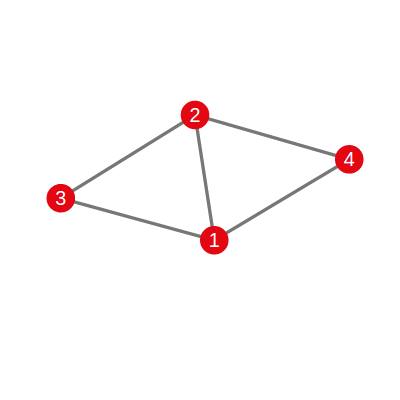
\includegraphics[scale=0.5]{./ej3/parte3/grafo1.jpg}
 	{\\Gráfico 3.3.1 - Grafo con número en nodos sin coloreo}
  \end{center}
  \vspace*{0.3cm}
  
En este grafo las opciones indicadas para coloreo fueron:\\
\begin{itemize}
\item Nodo 1 = Color 0 y Color 1
\item Nodo 2 = Color 0 y Color 2
\item Nodo 3 = Color 0 y Color 1
\item Nodo 4 = Color 0 y Color 2
\end{itemize}

Obteniendo  [0, 2, 1, 0] como resultado para la Heurística que se planteo y [1, 2, 0, 0] para el backtracking que enunciamos del ejercicio 2.\\

A continuación mostraremos como quedaría coloreado el grafo y como tendría que ser:\\

\vspace*{0.3cm} \vspace*{0.3cm}
  \begin{center}
 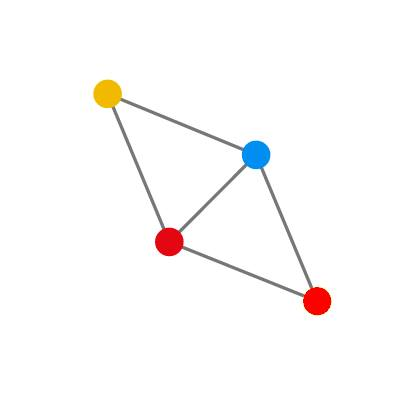
\includegraphics[scale=0.5]{./ej3/parte3/grafo1color.jpg}
 	{\\Gráfico 3.3.2 - Grafo con coloreo - Error de Heurística}
  \end{center}
  \vspace*{0.3cm}

  \vspace*{0.3cm} \vspace*{0.3cm}
  \begin{center}
 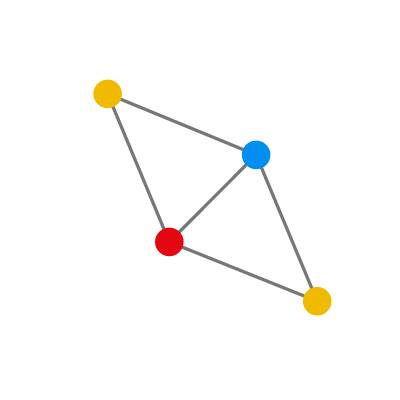
\includegraphics[scale=0.5]{./ej3/parte3/grafo1color2.jpg}
 	{\\Gráfico 3.3.3 - Grafo con coloreo - Solución Correcta}
  \end{center}
  \vspace*{0.3cm}
  
Luego, con el grafo:\\

\vspace*{0.3cm} \vspace*{0.3cm}
  \begin{center}
 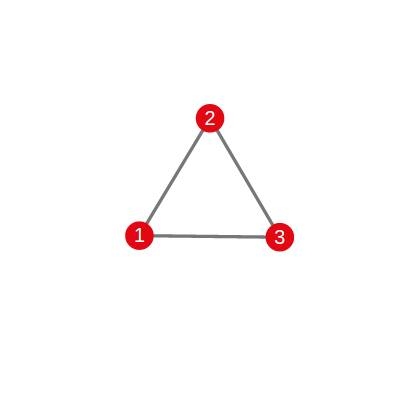
\includegraphics[scale=0.5]{./ej3/parte3/grafo2.jpg}
 	{\\Gráfico 3.3.4 - Grafo triangular con número en nodos sin coloreo}
  \end{center}
  \vspace*{0.3cm}
  
En este grafo las opciones indicadas para coloreo fueron:\\
\begin{itemize}
\item Nodo 1 = Color 1 y Color 2
\item Nodo 2 = Color 0 y Color 1
\item Nodo 3 = Color 0 y Color 1
\end{itemize}

Obteniendo  [1, 0, 0] como valor final para la Heurística que se planteo y [2, 0, 1] para el backtracking que enunciamos del ejercicio 2.\\

A continuación mostraremos un ejemplo de como quedó y como tendría que haber quedado coloreado el grafo:\\

\vspace*{0.3cm} \vspace*{0.3cm}
  \begin{center}
 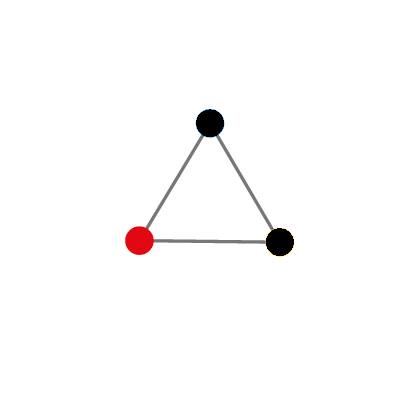
\includegraphics[scale=0.5]{./ej3/parte3/grafo2color.jpg}
 	{\\Gráfico 3.3.5 - Grafo con coloreo - Error de Heurística}
  \end{center}
  \vspace*{0.3cm}

  \vspace*{0.3cm} \vspace*{0.3cm}
  \begin{center}
 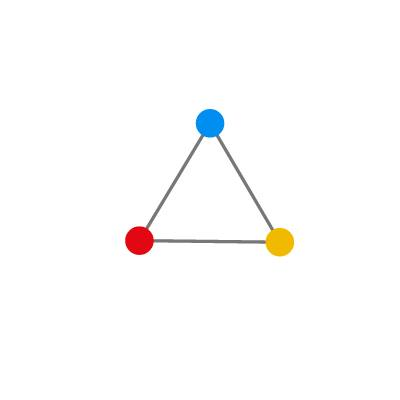
\includegraphics[scale=0.5]{./ej3/parte3/grafo2color2.jpg}
 	{\\Gráfico 3.3.6 - Grafo con coloreo - Solución Correcta}
  \end{center}
  \vspace*{0.3cm}
   
   
Por último, con el grafo:\\

\vspace*{0.3cm} \vspace*{0.3cm}
  \begin{center}
 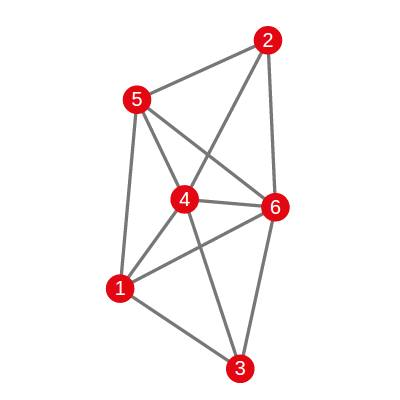
\includegraphics[scale=0.5]{./ej3/parte3/grafo3.jpg}
 	{\\Gráfico 3.3.7 - Grafo con número en nodos sin coloreo}
  \end{center}
  \vspace*{0.3cm}
  
En este grafo las opciones indicadas para coloreo fueron:\\
\begin{itemize}
\item Nodo 1 = Color 0 y Color 1
\item Nodo 2 = Color 0, Color 1 y Color 3
\item Nodo 3 = Color 2 y Color 3
\item Nodo 4 = Color 0, Color 2 y Color 3
\item Nodo 5 = Color 0, Color 1 y Color 3
\item Nodo 6 = Color 0, Color 2 y Color 3
\end{itemize}

Obteniendo [0, 1, 2, 3, 1, 0] como valor final para la Heurística que se planteo y [1, 1, 3, 0, 3, 2] para el backtracking que enunciamos del ejercicio 2.\\

A continuación mostraremos un ejemplo de como terminó quedando coloreado el grafo y como debería quedar:\\

\vspace*{0.3cm} \vspace*{0.3cm}
  \begin{center}
 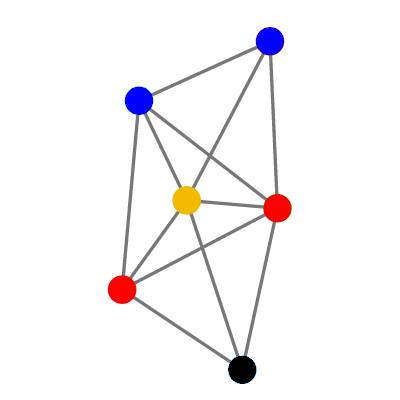
\includegraphics[scale=0.5]{./ej3/parte3/grafo3color.jpg}
 	{\\Gráfico 3.3.8 - Grafo con coloreo - Error de Heurística}
  \end{center}
  \vspace*{0.3cm}
  
  \vspace*{0.3cm} \vspace*{0.3cm}
  \begin{center}
 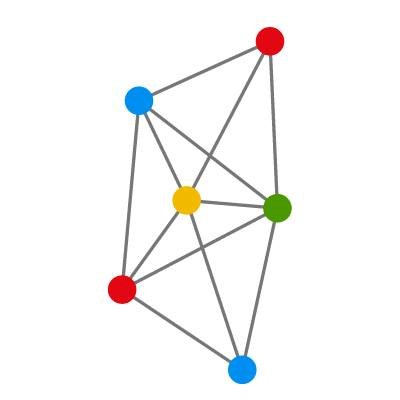
\includegraphics[scale=0.5]{./ej3/parte3/grafo3color2.jpg}
 	{\\Gráfico 3.3.9 - Grafo con coloreo - Solución Correcta}
  \end{center}
  \vspace*{0.3cm}
  